\documentclass{article}
\usepackage{color}
\usepackage{soul}
\usepackage{multirow}
\usepackage{pgfplots}
\usepackage{ifthen}
\usepackage[UTF8]{ctex}
\usepackage[left=2cm,right=2cm,top=2cm,bottom=2cm]{geometry}
\geometry{a4paper}
\usepackage{tikz}
\usetikzlibrary{chains}
\newcommand{\diff}{\mathop{}\!\mathrm{d}}
\usepackage{appendix} 
\usepackage{lipsum}
\usepackage{listings}
\usepackage{diagbox}
\usepackage{pdfpages}
\usepackage{xcolor}
\usepackage{pdflscape}
\usepackage{soul}
\usepackage{booktabs}
\usepackage{longtable}
\usepackage[most]{tcolorbox}
% \tcbuselibrary{breakable}
\newtcolorbox{mycolorbox}[1][]{
  sharp corners,
  colback=white, 
  colframe=black, 
  coltext=blue, 
  boxsep=5pt, 
  left=2pt, 
  right=2pt, 
  top=1pt, 
  bottom=1pt,
  breakable,
  #1 
}
\usepackage{subcaption}

% 通用设置
\lstset{
    %backgroundcolor=\color{white},
    backgroundcolor=\color{gray!20},
    basicstyle=\ttfamily,
    commentstyle=\color{darkgray}\ttfamily,
    stringstyle=\color{red},
    showstringspaces=false,
    numbers=left,
    numberstyle=\tiny\color{gray},
    stepnumber=1,
    numbersep=10pt,
    tabsize=4,
    showspaces=false,
    showtabs=false,
    frame=single,
    captionpos=b,
    breaklines=true,
    breakatwhitespace=false,
    escapeinside={\%*}{*)},
    xleftmargin=\parindent,
    xrightmargin=\parindent,
}
\lstdefinestyle{dockerstyle}{
    language=bash,
    keywordstyle=\color{blue}\bfseries,
    morekeywords={FROM, RUN, CMD, LABEL, EXPOSE, ENV, ADD, COPY, ENTRYPOINT, VOLUME, USER, WORKDIR, ARG, ONBUILD},
}
\lstdefinestyle{pythonstyle}{
    language=Python,
    keywordstyle=\color{blue}\bfseries,
    morekeywords={import, from, as, def, return, class, self, if, elif, else, while, for, try, except, with},
}
\lstdefinestyle{cstyle}{
    language=C,
    keywordstyle=\color{blue}\bfseries,
    morekeywords={size_t, printf},
}
\lstdefinestyle{bashstyle}{
    language=bash,
    keywordstyle=\color{blue}\bfseries,
    morekeywords={if, then, else, fi, for, in, do, done, echo, exit, return, function},
    commentstyle=\color{green}\ttfamily,
}
\usepackage{algorithm}
\usepackage{algpseudocode}
\renewcommand{\algorithmicrequire}{\textbf{Input:}}  
\renewcommand{\algorithmicensure}{\textbf{Output:}}  
\usepackage{amsmath}
\usepackage{amsthm}
\DeclareMathOperator{\sigm}{sigm}
\usepackage{graphicx}
\usepackage{float}
\renewcommand{\vec}[1]{\boldsymbol{#1}}
\usepackage{amssymb}
\usepackage{booktabs} 
\usepackage{hyperref}
\usepackage{titlesec}
\usepackage{caption}
\usepackage{fontspec}
\usepackage{xeCJK}
\setCJKmainfont{SimSun} 
\title{\Huge OpenMP并行编程实验报告}
\author{21121178 王士博}
\begin{document}
\maketitle
\section{实验环境}
\begin{enumerate}
    \item macOS Silicon:Apple M2 8核心 (@3.49GHz 4×高性能核心 + @2.42GHz 4×能效核心)。
    \item Windows Chip:Intel(R) Core(TM) i7-11800H 16线程 @ 4.60GHz。
    \item Docker:运行于非WSL2的Windows11上,镜像地址为\url{openmpp/openmpp-build:ubuntu}。
\end{enumerate}
\section{实验目的}
\begin{itemize}
    \item 并行计算的性能评估与分析;
    \item 并行计算在复杂运算中的加速效果;
    \item 并行编程技术的实际应用效果评价。
\end{itemize}
\section{实验步骤}
\begin{enumerate}
    \item 并行计算的性能评估与分析: 通过HelloWorld程序的串行执行与
    并行执行(不设置线程数以及设置8个线程)的对比分析,旨在揭示并行计算在不同线程
    配置下的性能变化及其对程序执行时间的影响。此实验目的在于评估并行计算相较于串行计
    算在处理简单任务时的效率提升,并分析线程数对执行效率的具体影响,以及探索默认线程
    配置下的系统表现。
    \item 并行计算在复杂运算中的加速效果: 通过编程实现大规模向量的矩阵乘法并
    行计算,并在不同的线程数(1、2、4、8、16、32)下评估执行时间,以及在不同操作系
    统环境(Windows, Linux及虚拟机下的Linux系统)中比较加速比。该实验目的在于深入分
    析并行计算在处理复杂数学运算时的性能提升,以及线程数与运行时间之间的关系,进一步理解
    操作系统环境对并行计算效率的影响。
    \item 并行编程技术的实际应用效果评价: 通过OpenMP实例估算Pi值的实验,调试并比较串行
    算法与四种不同的并行程序的加速比,检查并行编程是否有效提高计算效率。此外,探索其他实验
    内容,如私有变量和共有变量的性能对比,分析并行化的额外负担、线程负载均衡问题及线程同步
    问题。该实验目的旨在通过实际案例测试并行编程技术的应用效果,特别是在精确计算和资源调度
    方面的表现,为并行计算在科学研究和工程应用中的实践提供理论依据和技术支持。
    \item 根据上面对OpenMP的学习使用OpenMP进行更多的实验来加深印象和理解。
\end{enumerate}
\section{编程及结果分析}
\subsection{HelloWorld串行并行}
\indent 通过本次的实验可以发现,串行结构下运行之后只会打印一遍\texttt{HelloWorld},如果在
打印的语句之前加上\texttt{\#pragma omp parallel},则会打印8遍\texttt{HelloWorld}。
这是因为\texttt{\#pragma omp parallel}会创建一个并行区域,然后在这个区域中创建多个线程,
因为打印语句之前没有加\texttt{\#pragma omp single}或者\texttt{\#pragma omp master}进行
修饰,所以编译器会将这条打印语句分给所有的线程都执行一次,其中如果设置线程数为10,效果如图
\ref{fig:4}所示(因为本身CPU的核心数就为8),如果不设置线程数,效果如图\ref{fig:5}所示,
可以看到如果不使用线程数的设置,那么创建的并行区域会默认使用电脑的全部CPU核心进行多线程
的处理,此时$num\_thread=\$\{nproc\}$,如果设置线程数,那么编译器会按照设定的线程数进行
任务的分配。其中可以使用\texttt{single}和\texttt{master}子句来控制某个程序块中的代码只被一个线程执行一次,
其中\texttt{single}和\texttt{master}的区别在于\texttt{single}会被所有线程中的某一个执行一次
效果如图\ref{fig:1}所示,而\texttt{master}则是只会被线程号为0的主线程执行一次,效果如图\ref{fig:2}
所示。在后续的实验中,可以发现有些子句是互相嵌套的,比如\texttt{for}子句和\texttt{section(s)}子句
都自带\texttt{single}的特点,只会被执行一次。
\begin{figure}[H]
    \centering
    \begin{subfigure}[b]{0.3\textwidth}
        \centering
        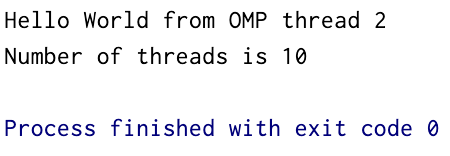
\includegraphics[width=\textwidth]{single.png}
        \caption{使用single的打印结果}
        \label{fig:1}
    \end{subfigure}
    \hfill
    \begin{subfigure}[b]{0.3\textwidth}
        \centering
        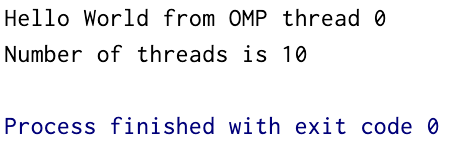
\includegraphics[width=\textwidth]{master.png}
        \caption{使用master的打印结果}
        \label{fig:2}
    \end{subfigure}
    \hfill
    \begin{subfigure}[b]{0.3\textwidth}
        \centering
        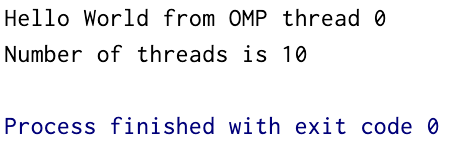
\includegraphics[width=\textwidth]{master.png}
        \caption{串行的打印结果}
        \label{fig:3}
    \end{subfigure}

    \begin{subfigure}[b]{0.45\textwidth}
        \centering
        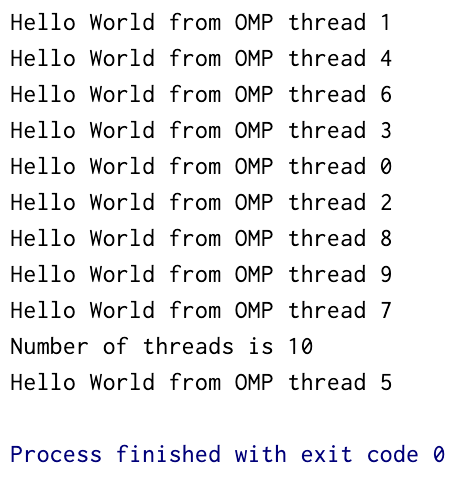
\includegraphics[width=\textwidth]{set10.png}
        \caption{设置线程数为10的打印结果}
        \label{fig:4}
    \end{subfigure}
    \hfill
    \begin{subfigure}[b]{0.45\textwidth}
        \centering
        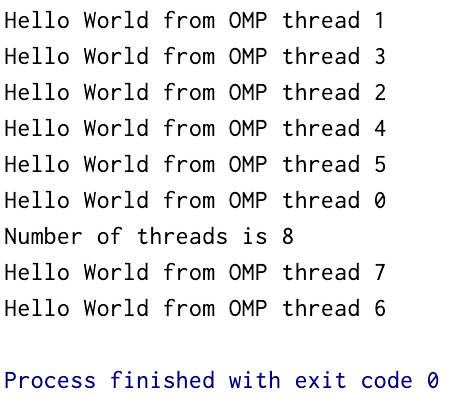
\includegraphics[width=\textwidth]{noset.png}
        \caption{不设置线程数的打印结果}
        \label{fig:5}
    \end{subfigure}
    \caption{不同设置下的HelloWorld的打印结果}
\end{figure}
\subsection{关于矩阵乘法的实验}
下面是本次实验使用的所有规格设备的运行串行矩阵乘法的用时,也是Baseline的数据。
\texttt{Ubuntu(n)}代表了运行在Windows上的Docker镜像,这里的镜像地址都来自于实验环境
中的Docker镜像地址,其中的\texttt{n}代表的是核心数,通过Docker Desktop进行修改。
其中红色标出了Baseline中在$1000\times1000$,$2000\times2000$和$3000\times3000$大小矩阵的
最快运行时间的设备。去除程序运行的偶然性,基本的运行时间误差在5\%左右,但是可以看出镜像运行的速度
是远高于宿主机和其他设备的这里考虑到Docker的特点可以总结出以下几点原因:
\begin{enumerate}
    \item \textbf{资源限制}:Docker 容器可以配置 CPU 和内存使用限制。如果宿主机上运行很多其他程序,这些程序可能会竞争资源,导致你的程序运行缓慢。而在 Docker 容器中,你的程序可能通过资源限制获得了保证的 CPU 时间和内存,从而运行得更快。
    \item \textbf{文件系统缓存}:Docker 容器使用宿主机的文件系统,但也可以配置为使用特定的存储驱动来优化读写操作。在某些情况下,这可能会导致容器内的文件操作比直接在宿主机上执行时更高效。
    \item \textbf{内核优化}:Docker 容器直接运行在宿主机的内核上,但某些内核调优(如 TCP/IP 堆栈调优)可能只对容器内部的程序有益,这取决于 Docker 的配置和宿主机的系统设置。
  \end{enumerate}
\begin{table}[H]
    \centering
    \label{tab:1}
    \begin{tabular}{|c|c|c|c|}
    \hline
    \diagbox{Device}{Size} & 1000 & 2000 & 3000 \\ \hline
    Mac OS & 3.62 & 31.74 & 112.17 \\ \hline
    Windows & 2.71 & 31.91 & 143.90 \\ \hline
    Ubuntu (4) & 2.14 & {\heiti \textcolor{red}{\textbf{\textit{22.66}}}} & 82.43 \\ \hline
    Ubuntu (8) & {\heiti \textcolor{red}{\textbf{\textit{2.12}}}} & 22.84 & 82.11 \\ \hline
    Ubuntu (16) & 2.14 & 23.03 & {\heiti \textcolor{red}{\textbf{\textit{81.96}}}} \\ \hline
    \end{tabular}
    \caption{不同设备运行串行矩阵乘法的时间(注:Ubuntu(n)中n代表的是核心数,这里的Ubuntu没有特殊说明都是运行在Windows上的镜像)}
\end{table}
\begin{table}[H]
    \centering
    \label{tab:2}
    \begin{tabular}{cccc}
    \toprule
    \textbf{Thread} & \textbf{Matrix Size} & \textbf{Use Reduction(s)} & \textbf{No Reduction(s)} \\
    \midrule
    \multirow{3}{*}{1} & 1000 & 3.12 (0.87) & 2.47 (1.1) \\
    & 2000 & 35.57 (0.9) & 32.25 (0.99) \\
    & 3000 & 150.29 (0.96) & 143.59 (1.0) \\
    \midrule
    \multirow{3}{*}{2} & 1000 & 1.66 (1.63) & 1.39 (1.95) \\
    & 2000 & 18.61 (1.71) & 16.50 (1.93) \\
    & 3000 & 77.42 (1.86) & 73.27 (1.96) \\
    \midrule
    \multirow{3}{*}{4} & 1000 & 0.98 (2.77) & 0.92 (2.95) \\
    & 2000 & 9.70 (3.29) & 8.85 (3.61) \\
    & 3000 & 41.42 (3.47) & 40.05 (3.59) \\
    \midrule
    \multirow{3}{*}{8} & 1000 & 0.62 (4.37) & 0.55 (4.93) \\
    & 2000 & 5.94 (5.37) & 5.40 (5.91) \\
    & 3000 & 25.26 (5.7) & 24.21 (5.94) \\
    \midrule
    \multirow{3}{*}{16} & 1000 & 0.53 (5.11) & 0.48 (5.65) \\
    & 2000 & 6.08 (5.25) & 5.81 (5.49) \\
    & 3000 & 22.17 (6.49) & 22.03 (6.53) \\
    \midrule
    \multirow{3}{*}{32} & 1000 & 0.53 (5.11) & 0.47 (5.77) \\
    & 2000 & 5.86 (5.45) & 5.67 (5.63) \\
    & 3000 & 22.29 (6.46) & 21.72 (6.63) \\
    \bottomrule
    \end{tabular}
    \caption{Windows和macOS不同大小矩阵和设定的线程数运行时间对比(包含加速比)}
\end{table}

首先测试了是否使用reduction子句优化最内层的循环进行求和可以提高程序的运行速度。如表\ref{tab:2}所示,
可以看到原本应该加速的程序并没有被加速,反而却整体运行速度都变慢了,总结有如下几点原因:
\begin{enumerate}
    \item \textbf{reduction操作的开销:} \texttt{reduction}子句由于需要为每个线程维护reduction变量的私有副本并在并行区域结束时合并它们,引入了额外的开销。在最内层循环的情况下,这种开销可能会抵消并行化累加操作的好处。
    \item \textbf{频繁的同步:} 在最内层循环中利用\texttt{reduction}会导致在循环结束时频繁的同步点,因为线程需要更新全局累加器。这种频繁的同步可能会阻碍并行执行效率,特别是当循环迭代计算量不大时。
    \item \textbf{缓存和内存带宽的次优利用:} 最内层循环中的并行reduction可能导致缓存和内存带宽的使用不佳,因为该操作可能阻止有效地利用空间和时间局部性。结果可能是增加了缓存未命中和内存流量,这可能会减慢计算速度。
\end{enumerate}
\begin{table}[H]
    \centering
    \begin{tabular}{cccc}
    \toprule
    \textbf{Thread} & \textbf{Matrix Size} & \textbf{MacOS(s)} & \textbf{Windows(s)} \\
    \midrule
    \multirow{3}{*}{1} & 1000 & 3.61 & 2.47 \\
                       & 2000 & 30.72 & 32.25 \\
                       & 3000 & 107.18 & 143.59 \\
    \midrule
    \multirow{3}{*}{2} & 1000 & 1.85 & 1.39 \\
                       & 2000 & 15.92 & 16.50 \\
                       & 3000 & 56.11 & 73.27 \\
    \midrule
    \multirow{3}{*}{4} & 1000 & 0.98 & 0.92 \\
                       & 2000 & 8.20 & 8.85 \\
                       & 3000 & 29.35 & 40.05 \\
    \midrule
    \multirow{3}{*}{8} & 1000 & 0.65 & 0.55 \\
                       & 2000 & 5.90 & 5.40 \\
                       & 3000 & 23.73 & 24.21 \\
    \midrule
    \multirow{3}{*}{16} & 1000 & 0.64 & 0.48 \\
                        & 2000 & 5.63 & 5.81 \\
                        & 3000 & 23.82 & 22.03 \\
    \midrule
    \multirow{3}{*}{32} & 1000 & 0.64 & 0.47 \\
                        & 2000 & 5.58 & 5.67 \\
                        & 3000 & 23.20 & 21.72 \\
    \bottomrule
    \end{tabular}
    \caption{Windows和macOS不同大小矩阵和设定的线程数运行时间对比}
\end{table}

然后本实验测试了在八核心的macOS和16核心的Windows
\begin{table}[H]
    \centering
    \begin{tabular}{|c|c|c|c|}
    \hline
    \diagbox{nproc}{thread} & 4 & 8 & 16 \\ \hline
    1 & 22.93 & 22.74 & 22.83  \\ \hline
    2 & 13.59 & 13.05 & 12.83  \\ \hline
    4 & {\heiti \textcolor{red}{\textbf{\textit{7.11}}}} & 7.15 & 7.53  \\ \hline
    8 & 6.88 & {\heiti \textcolor{red}{\textbf{\textit{4.38}}}} & 4.28  \\ \hline
    16 & 6.62 & 4.30 & {\heiti \textcolor{red}{\textbf{\textit{3.18}}}}  \\ \hline
    32 & 7.08 & 4.39 & 3.17  \\ \hline
    \end{tabular}
    \caption{在不同的nproc和线程数下的性能数据(sec)}
\end{table}
\begin{figure}
    \centering
    \begin{subfigure}[b]{0.45\textwidth}
        \centering
        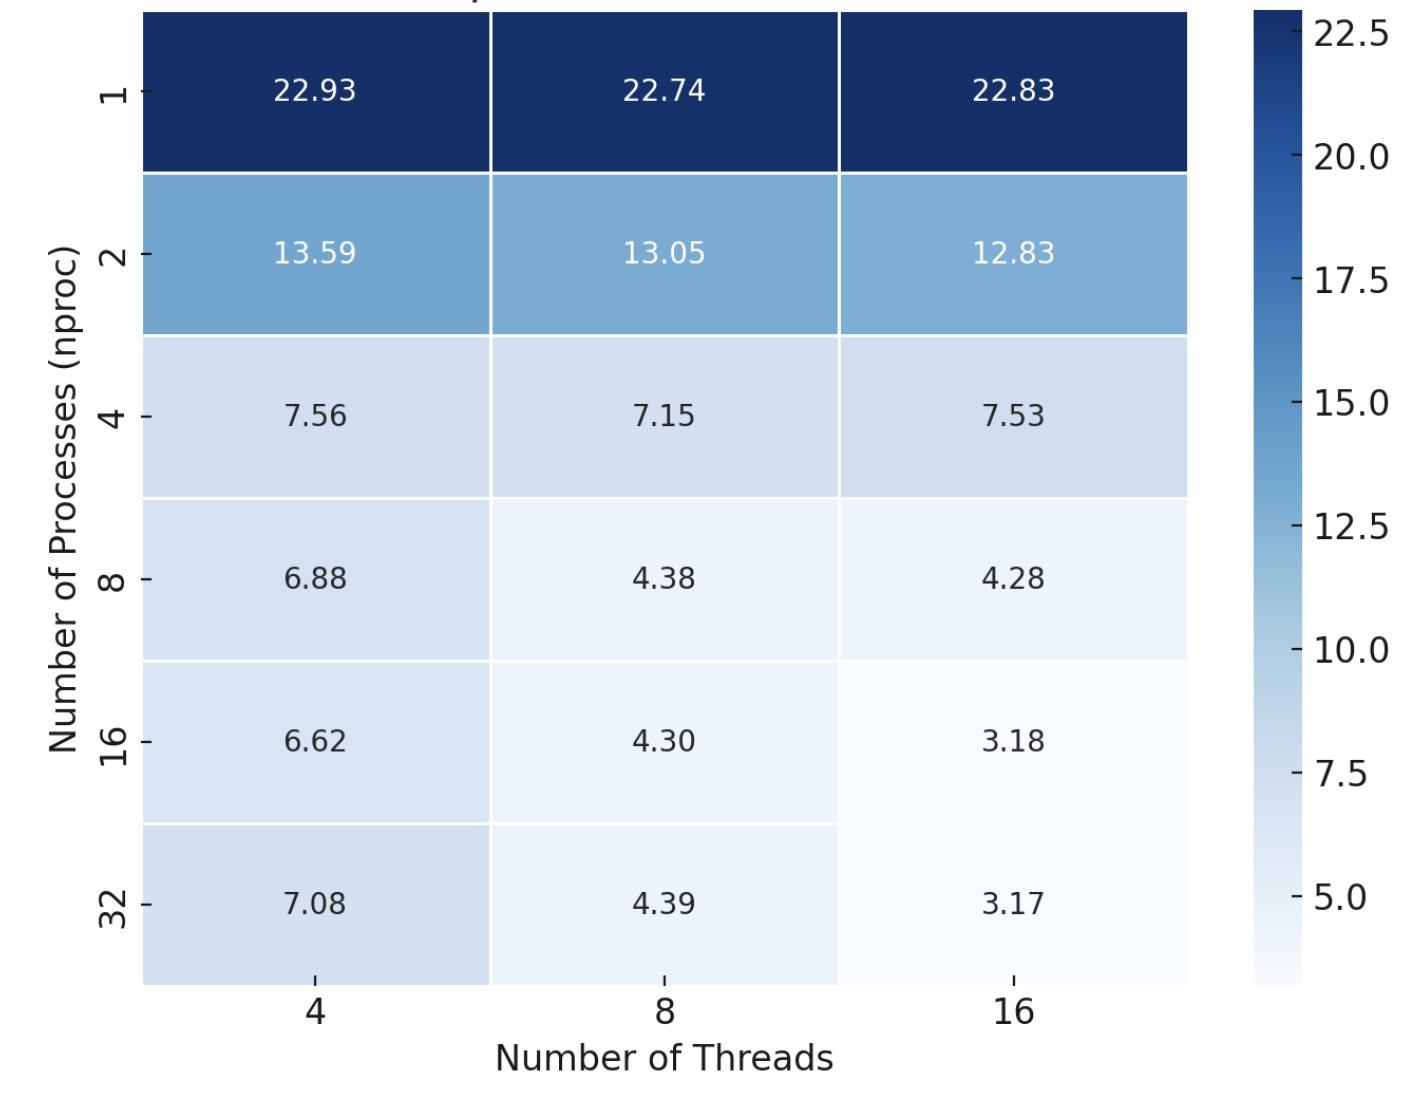
\includegraphics[width=\textwidth]{heatmap.png}
        \caption{nprco和thread热力图}
    \end{subfigure}
    \hfill
    \begin{subfigure}[b]{0.45\textwidth}
        \centering
        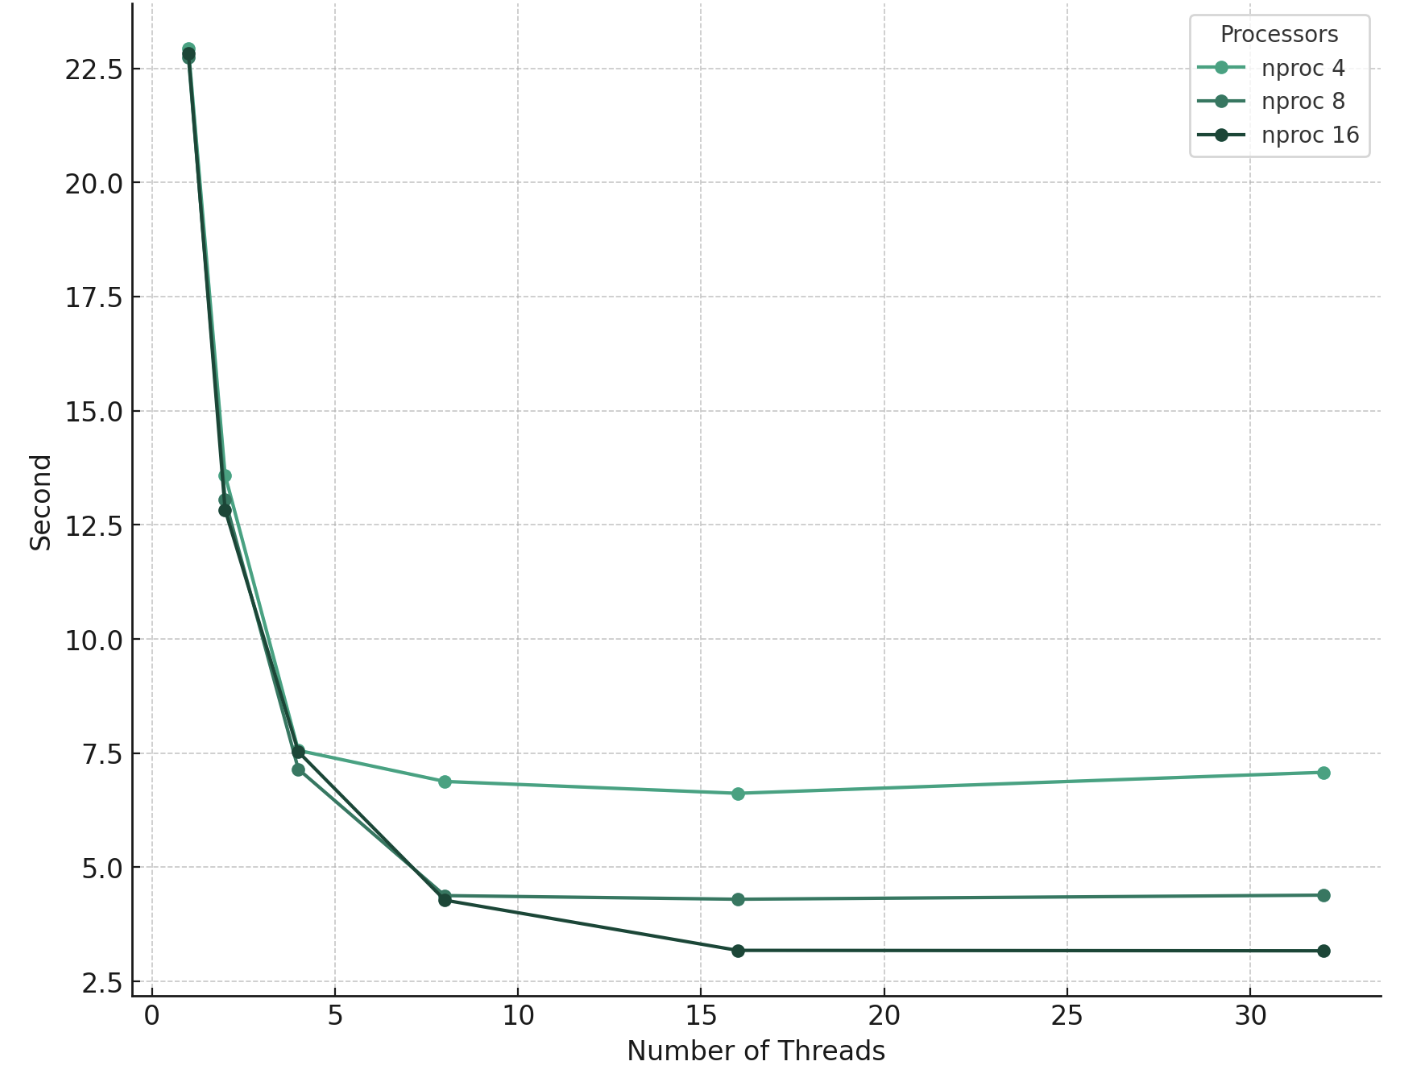
\includegraphics[width=\textwidth]{statistic.png}
        \caption{nproc和thread的折线图}
    \end{subfigure} 
\end{figure}
\subsection{计算$\pi$值的实验}

\subsection{}
\section{实验感想}
\newpage
\appendix
\section{附录}
\noindent
\begin{minipage}[t]{0.45\textwidth}
    \begin{lstlisting}[style=cstyle,caption={串行Helloworld}]
#include"omp.h"
#include"stdio.h"
int main(){
    int nthreads,tid;
    tid=omp_get_thread_num();
    printf("Hello World from OMP thread %d\n",tid);
    if(tid==0)
    {
        nthreads=omp_get_num_threads();
        printf("Number of threads is %d\n",nthreads);
    }
}
    \end{lstlisting}
\end{minipage}
\hfill 
\begin{minipage}[t]{0.45\textwidth}
    \begin{lstlisting}[style=cstyle,caption={不设线程并行Helloworld}]
#include"omp.h"
#include"stdio.h"
int main(){
    int nthreads,tid;
    #pragma omp parallel private(nthreads,tid)
    {
        tid=omp_get_thread_num();
        printf("Hello World from OMP thread %d\n",tid);
        if(tid==0)
        {
            nthreads=omp_get_num_threads();
            printf("Number of threads is %d\n",nthreads);
        }
    }
}
    \end{lstlisting}
\end{minipage}
\begin{lstlisting}[style=cstyle,caption={设置10个线程并行Helloworld}]
#include"omp.h"
#include"stdio.h"
int main(){
    int nthreads,tid;
    omp_set_num_threads(10);
 #pragma omp parallel private(nthreads,tid)
    {
        tid=omp_get_thread_num();
        printf("Hello World from OMP thread %d\n",tid);
        if(tid==0)
        {
            nthreads=omp_get_num_threads();
            printf("Number of threads is %d\n",nthreads);
        }
    }
}
\end{lstlisting}
\begin{lstlisting}[style=cstyle,caption={串行矩阵乘法}]
#include <stdio.h>
#include <stdlib.h>
#include <time.h>
void generateMatrix(double* matrix, int size) {
    for (int i = 0; i < size * size; i++) {
        matrix[i] = rand() % 10;
    }
}
void multiplyMatrices(double* a, double* b, double* result, int size) {
    for (int row = 0; row < size; row++) {
        for (int col = 0; col < size; col++) {
            double sum = 0.0;
            for (int k = 0; k < size; k++) {
                sum += a[row * size + k] * b[k * size + col];
            }
            result[row * size + col] = sum;
        }
    }
}
int main() {
    srand(time(NULL));
    int sizes[] = {1000, 2000, 3000};
    for (int index = 0; index < 3; index++) {
        int size = sizes[index];
        printf("Generating and multiplying matrices of size %dx%d.\n", size, size);
        double* a = malloc(size * size * sizeof(double));
        double* b = malloc(size * size * sizeof(double));
        double* result = malloc(size * size * sizeof(double));
        if (a == NULL || b == NULL || result == NULL) {
            printf("Memory allocation failed\n");
            exit(1);
        }
        generateMatrix(a, size);
        generateMatrix(b, size);
        clock_t start = clock();
        multiplyMatrices(a, b, result, size);
        clock_t end = clock();
        double time_spent = (double)(end - start) / CLOCKS_PER_SEC; // 计算运行时间
        printf("Done with size %dx%d. Time: %.2f seconds.\n", size, size, time_spent);
        free(a);
        free(b);
        free(result);
    }
    return 0;
}
\end{lstlisting}
\begin{lstlisting}[style=cstyle,caption={并行矩阵乘法}]
#include <stdio.h>
#include <stdlib.h>
#include <time.h>
#include <omp.h>
void generateMatrix(double* matrix, int size) {
    for (int i = 0; i < size * size; i++) {
        matrix[i] = rand() % 10;
    }
}
void multiplyMatrices(double* a, double* b, double* result, int size) {
    int i,j,k;
#pragma omp parallel for shared(a, b, result) private(i, j, k) schedule(dynamic, 10) num_threads(32)
    for (i = 0; i < size; i++) {
        for (j = 0; j < size; j++) {
            double sum = 0.0;
            for (k = 0; k < size; k++) {
                sum += a[i * size + k] * b[k * size + j];
            }
            result[i * size + j] = sum;
        }
    }
}
int main() {
    srand(time(NULL));

    int sizes[] = {1000, 2000, 3000};
    for (int index = 0; index < 3; index++) {
        int size = sizes[index];
        printf("Generating and multiplying matrices of size %dx%d.\n", size, size);

        double* a = malloc(size * size * sizeof(double));
        double* b = malloc(size * size * sizeof(double));
        double* result = malloc(size * size * sizeof(double));

        if (a == NULL || b == NULL || result == NULL) {
            printf("Memory allocation failed\n");
            exit(1);
        }

        generateMatrix(a, size);
        generateMatrix(b, size);

        double start = omp_get_wtime();
        multiplyMatrices(a, b, result, size);
        double end = omp_get_wtime();

        double time_spent = end - start;
        printf("Done with size %dx%d. Time: %.2f seconds.\n", size, size, time_spent);

        free(a);
        free(b);
        free(result);
    }

    return 0;
}
\end{lstlisting}
\begin{lstlisting}[style=cstyle,caption={串行$\pi$值计算}]
#include <stdio.h>
#include <time.h>
static long num_steps = 100000;
double step;
int main() {
    int i;
    double x, pi, sum = 0.0;
    clock_t start, end;
    double cpu_time_used;
    step = 1.0 / (double)num_steps;
    start = clock();
    for (i = 0; i < num_steps; i++) {
        x = (i + 0.5) * step;
        sum = sum + 4.0 / (1.0 + x * x);
    }
    pi = step * sum;
    end = clock();
    cpu_time_used = ((double) (end - start)) / CLOCKS_PER_SEC;

    printf("Value of Pi = %.16f\n", pi);
    printf("Time taken: %.8f seconds\n", cpu_time_used);

    return 0;
}
\end{lstlisting}
\begin{lstlisting}[style=cstyle,caption={并行$\pi$值计算1}]
#include <stdio.h>
#include <omp.h>
static long num_steps = 100000;
double step;
#define NUM_THREADS 2
int main() {
    int i;
    double pi, sum = 0.0;
    step = 1.0 / (double) num_steps;
    omp_set_num_threads(NUM_THREADS);
    double start_time = omp_get_wtime();
#pragma omp parallel private(i) reduction(+:sum)
    {
        double x;
        int id = omp_get_thread_num();
        for (i = id; i < num_steps; i += NUM_THREADS) {
            x = (i + 0.5) * step;
            sum += 4.0 / (1.0 + x * x);
        }
    }
    pi = sum * step;
    double end_time = omp_get_wtime();
    printf("Value of Pi = %.16f\n", pi);
    printf("Time taken: %.8f seconds\n", end_time - start_time);
    return 0;
} 
\end{lstlisting}
\begin{lstlisting}[style=cstyle,caption={并行$\pi$值计算2}]
#include <stdio.h>
#include <omp.h>
static long num_steps = 100000;
double step;
#define NUM_THREADS 2
int main() {
    int i;
    double pi = 0.0;
    step = 1.0 / (double) num_steps;
    omp_set_num_threads(NUM_THREADS);
    double start_time = omp_get_wtime();
#pragma omp parallel
    {
        double x;
        int id = omp_get_thread_num();
        double partial_sum = 0.0;
#pragma omp for
        for (i = 0; i < num_steps; i++) {
            x = (i + 0.5) * step;
            partial_sum += 4.0 / (1.0 + x * x);
        }
#pragma omp critical
        pi += partial_sum * step;
    }

    double end_time = omp_get_wtime();
    printf("Value of Pi = %.16f\n", pi);
    printf("Time taken: %.8f seconds\n", end_time - start_time);
    return 0;
}  
\end{lstlisting}
\begin{lstlisting}[style=cstyle,caption={并行$\pi$值计算3}]
#include <stdio.h>
#include <omp.h>
static long num_steps = 100000;
double step;
#define NUM_THREADS 2
int main() {
    int i, id;
    double x, sum, pi = 0.0;
    step = 1.0 / (double) num_steps;
    omp_set_num_threads(NUM_THREADS);
    double start_time = omp_get_wtime();
#pragma omp parallel private(i, id, x, sum)
    {
        id = omp_get_thread_num();
        sum = 0.0;
        for (i = id; i < num_steps; i += NUM_THREADS) {
            x = (i + 0.5) * step;
            sum += 4.0 / (1.0 + x * x);
        }
#pragma omp critical
        pi += sum * step;
    }
    double end_time = omp_get_wtime();
    printf("Pi = %.16f\n", pi);
    printf("Time taken: %.8f seconds\n", end_time - start_time);
    return 0;
}
\end{lstlisting}
\begin{lstlisting}[style=cstyle,caption={并行$\pi$值计算4}]
#include <stdio.h>
#include <omp.h>
static long num_steps = 100000;
double step;
#define NUM_THREADS 2
int main() {
    int i;
    double x, pi, sum = 0.0;
    step = 1.0 / (double) num_steps;
    omp_set_num_threads(NUM_THREADS);
    double start_time = omp_get_wtime();
#pragma omp parallel for reduction(+:sum) private(x)
    for (i = 0; i < num_steps; i++) {
        x = (i + 0.5) * step;
        sum += 4.0 / (1.0 + x * x);
    }
    pi = step * sum;
    double end_time = omp_get_wtime();
    printf("Pi = %.16f\n", pi);
    printf("Time taken: %.8f seconds\n", end_time - start_time);

    return 0;
}
\end{lstlisting}
\end{document}